% =============================================================================
% Apresentação de defesa — baseada na dissertação
% Detecção Automatizada de Ocultações Estelares com Machine Learning
% Compila em pdfLaTeX (Overleaf-compatível). Imagens em figs/.
% Filosofia: pouco texto, muito gráfico, explicação verbal do apresentador.
% =============================================================================
\documentclass[aspectratio=169]{beamer}

\usetheme{Boadilla}
\usecolortheme{seahorse}
\setbeamertemplate{navigation symbols}{}      % remove ícones de navegação
\setbeamertemplate{caption}{\insertcaption}    % legendas limpas

\usepackage[T1]{fontenc}
\usepackage[utf8]{inputenc}
\usepackage[brazil]{babel}
\usepackage{graphicx}
\usepackage{booktabs}
\usepackage{amsmath}
\usepackage{xcolor}

\graphicspath{{figs/}}

% Cor de destaque para números/achados
\definecolor{destaque}{RGB}{176,0,32}
\newcommand{\hl}[1]{{\color{destaque}\textbf{#1}}}

% --- Metadados ---
\title[Detecção de Ocultações com ML]{Pipeline para Detecção Automatizada de\\ Ocultações Estelares em Curvas de Luz\\ com Técnicas de \textit{Machine Learning}}
\author[T.\ Laidler]{Thiago Laidler Vidal Cunha}
\institute[ON]{Orientador: Dr.\ Júlio Camargo \\ Observatório Nacional}
\date{Julho de 2026}

\begin{document}

% ---------------------------------------------------------------- TÍTULO
\begin{frame}[plain]
  \titlepage
\end{frame}

% ---------------------------------------------------------------- ROTEIRO
\begin{frame}{Roteiro}
  \begin{columns}[T]
    \column{0.5\textwidth}
    \begin{enumerate}
      \item Motivação
      \item O problema
      \item A \textit{pipeline}
      \item Dados e características
    \end{enumerate}
    \column{0.5\textwidth}
    \begin{enumerate}\setcounter{enumi}{4}
      \item Resultados
      \item Estudo de caso: Quaoar
      \item Conclusões
    \end{enumerate}
  \end{columns}
\end{frame}

% ================================================================ 1. MOTIVAÇÃO
\section{Motivação}

\begin{frame}{Ocultações estelares: medir o invisível}
  \begin{columns}[c]
    \column{0.52\textwidth}
    \begin{itemize}
      \item Um corpo do Sistema Solar cruza a frente de uma estrela.
      \item A \alert{curva de luz} revela tamanho, forma, anéis, atmosfera.
      \item Precisão de \hl{quilômetros} a dezenas de UA.
    \end{itemize}
    \column{0.48\textwidth}
    \centering
    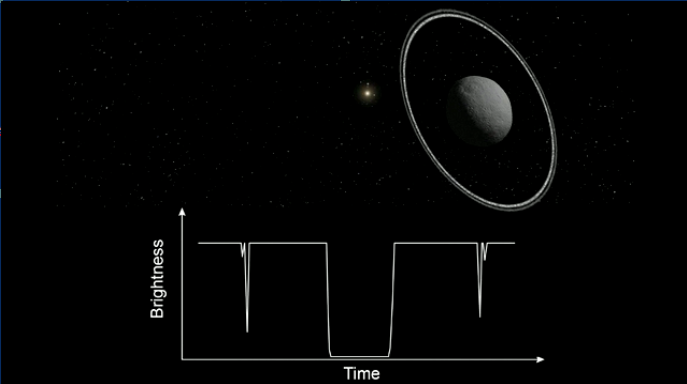
\includegraphics[width=\linewidth]{ocultacao_ilustracao.png}
  \end{columns}
  \vfill
  {\footnotesize Crédito: Lucie Maquet (2014) --- sistema de anéis de Chariklo.}
\end{frame}

\begin{frame}{Dois níveis de exigência}
  \begin{block}{O mínimo}
    Detectar a \textbf{queda profunda} do corpo principal --- sinal forte, fácil.
  \end{block}
  \begin{block}{O que importa de verdade}
    Não perder os \alert{sinais sutis} --- anéis, atmosferas tênues.
  \end{block}
  \vfill
  \centering
  \hl{Os anéis de Quaoar} foram descobertos só em uma \textbf{revisita} dos dados.\\
  {\footnotesize Um alerta automático nesses casos pode salvar uma descoberta.}
\end{frame}

% ================================================================ 2. PROBLEMA
\section{O problema}

\begin{frame}{O gargalo: \textit{big data} em ocultações}
  \begin{itemize}
    \item Redes de telescópios $+$ Gaia $\Rightarrow$ volume massivo de curvas.
    \item Triagem manual não escala.
    \item Ruído atmosférico/instrumental \textbf{imita} ocultações.
  \end{itemize}
  \vfill
  \begin{exampleblock}{Formulação}
    \centering
    \textbf{Classificação binária:} cada curva $\rightarrow$ vetor de \textit{features} $\rightarrow$
    \alert{positiva} (ocultação) ou \alert{negativa}.
  \end{exampleblock}
  \vfill
  {\footnotesize Abordagem: \textit{features} clássicas $+$ \textit{ensembles} de árvores --- interpretáveis, não caixa-preta.}
\end{frame}

% ================================================================ 3. PIPELINE
\section{Pipeline}

\begin{frame}{A \textit{pipeline} em cinco etapas}
  \centering
  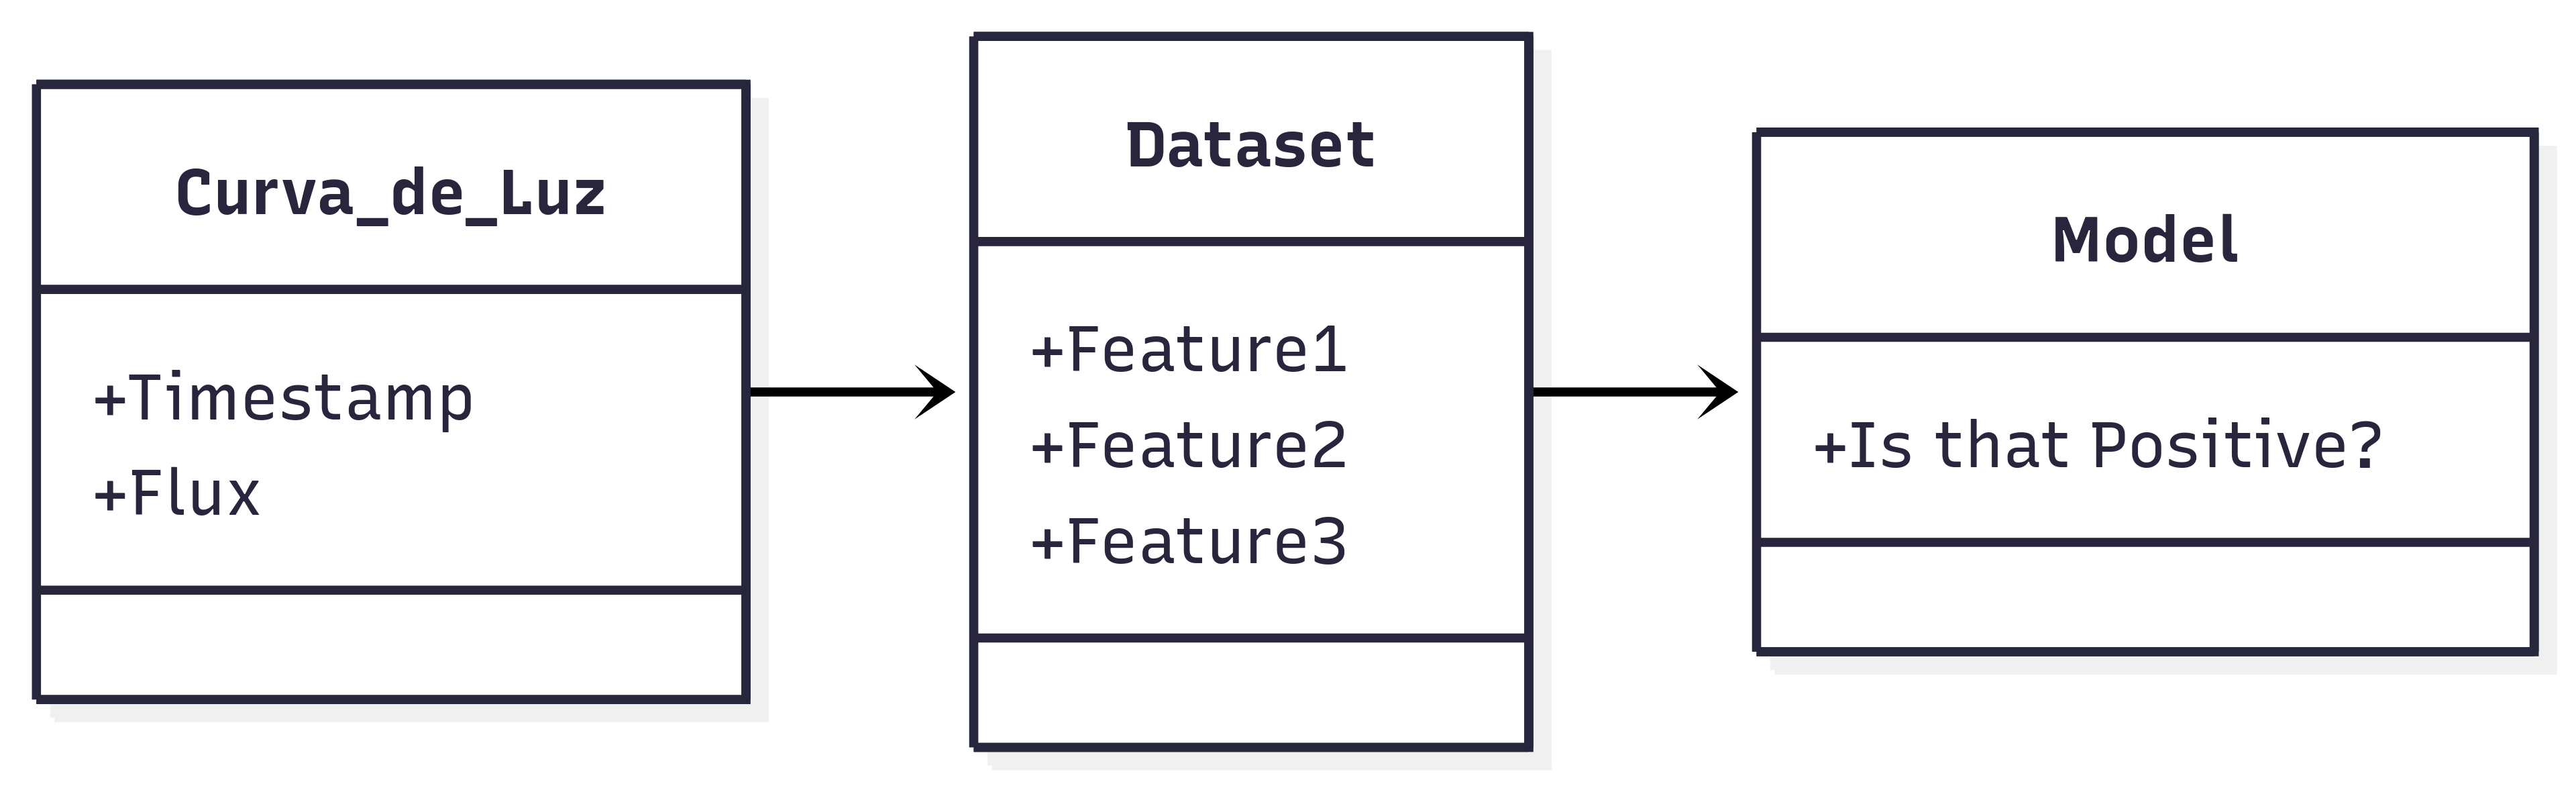
\includegraphics[width=0.92\linewidth]{pipeline.png}
  \vfill
  {\footnotesize Aquisição $\to$ normalização $\to$ construção do \textit{dataset} $\to$
  extração de \textit{features} $\to$ treino/avaliação.}
\end{frame}

% ================================================================ 4. DADOS
\section{Dados e características}

\begin{frame}{O conjunto de dados: \hl{1693 curvas}}
  \centering
  \begin{tabular}{lc}
    \toprule
    \textbf{Fonte} & \textbf{Quantidade} \\
    \midrule
    Positivas do banco (VizieR, Grupo do Rio) & 802 \\
    Sintéticas negativas (simulador físico)   & 702 \\
    Negativos artificiais (recorte manual)    & 186 \\
    Negativas do banco                        & 3 \\
    \midrule
    \textbf{Total} & \textbf{1693} \quad(802 pos. / 891 neg.) \\
    \bottomrule
  \end{tabular}
  \vfill
  \begin{itemize}
    \item Divisão estratificada por curva (sem vazamento).
    \item \alert{Limitação assumida:} 78\% das negativas são sintéticas.
  \end{itemize}
\end{frame}

\begin{frame}{De curva a vetor: \textit{features} de domínio}
  \begin{columns}[c]
    \column{0.54\textwidth}
    {\footnotesize
    \begin{itemize}
      \item Profundidade e SNR do \textit{dip}
      \item \textit{Max drawdown}, mínimo do Savitzky--Golay
      \item Distância entre centróides do K-means
      \item Testes estatísticos entre quartis ($t$, K--S)
      \item Razões de $\chi^2$ (constante vs.\ poço)
    \end{itemize}}
    \column{0.46\textwidth}
    \centering
    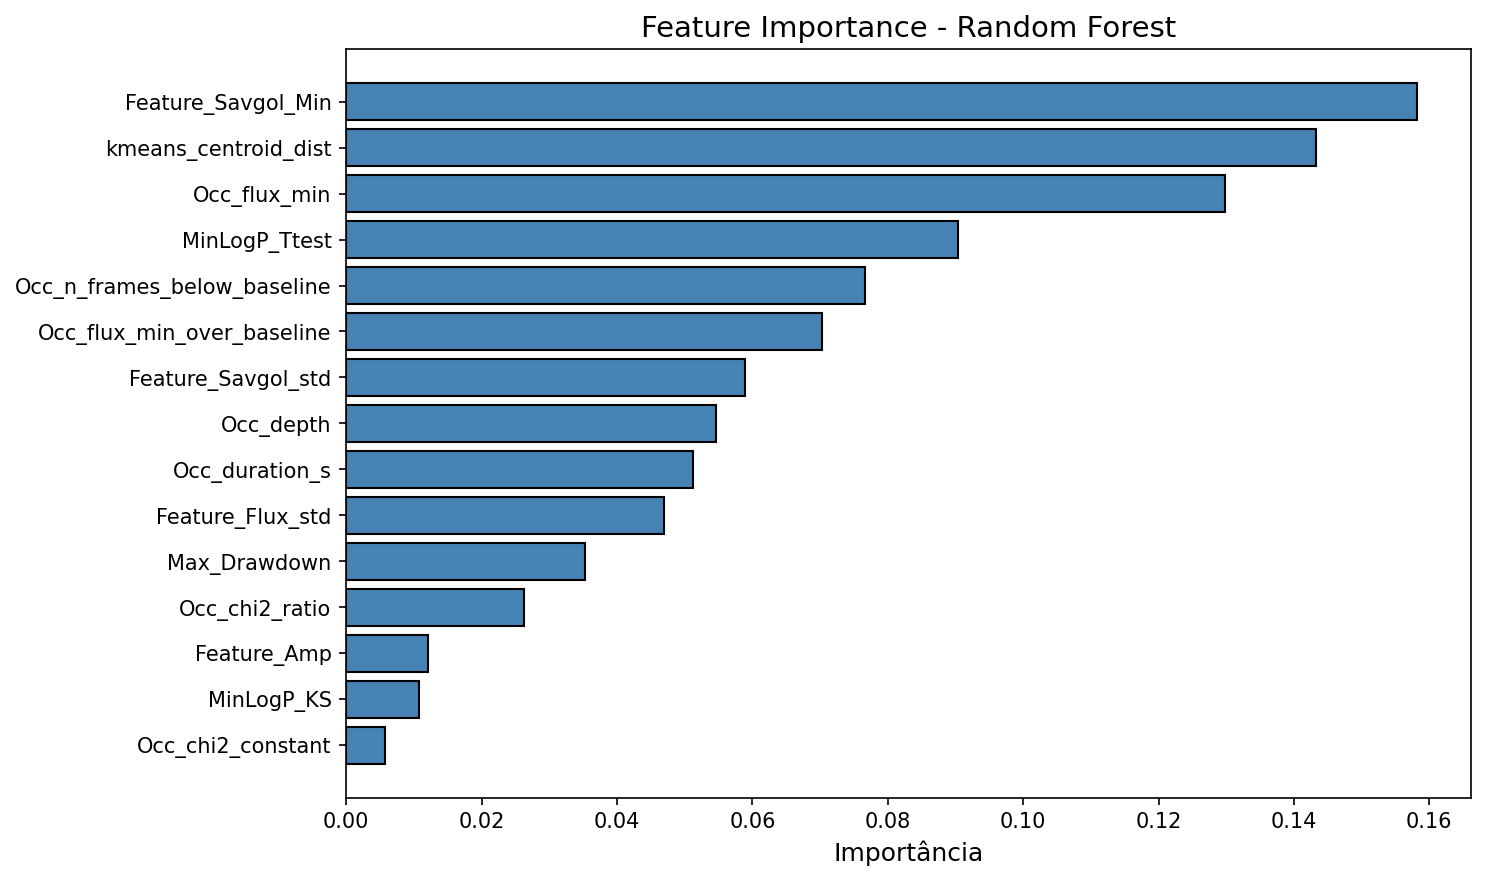
\includegraphics[width=\linewidth]{feat_importance_rf.png}\\
    {\scriptsize Importância (Random Forest, Exp.~1).}
  \end{columns}
  \vfill
  \centering Quatro classificadores: \textbf{Regressão Logística, Random Forest, XGBoost, CatBoost}.
\end{frame}

% ================================================================ 5. RESULTADOS
\section{Resultados}

\begin{frame}{Seis experimentos, desempenho estável}
  \centering
  {\scriptsize
  \begin{tabular}{lcccccc}
    \toprule
    \textbf{F1-score} & \textbf{Exp.1} & \textbf{Exp.2} & \textbf{Exp.3} & \textbf{Exp.4} & \textbf{Exp.5} & \textbf{Exp.6} \\
     & \tiny 28 f. & \tiny 11 f. & \tiny teste real & \tiny 14 f. & \tiny 13 f. & \tiny 12 f. \\
    \midrule
    Random Forest    & \textbf{0,9937} & 0,9874 & 0,9803 & 0,9874 & \textbf{0,9905} & \textbf{0,9906} \\
    XGBoost          & 0,9844 & \textbf{0,9906} & \textbf{0,9821} & 0,9875 & 0,9843 & \textbf{0,9906} \\
    CatBoost         & 0,9906 & 0,9905 & 0,9784 & \textbf{0,9906} & 0,9873 & 0,9874 \\
    Regressão Log.   & 0,9873 & 0,9841 & 0,9746 & 0,9873 & 0,9873 & 0,9873 \\
    \bottomrule
  \end{tabular}}
  \vfill
  \begin{itemize}\footnotesize
    \item \hl{F1 $\approx$ 0,99} e AUC-ROC $>$ 0,998 em todos os cenários.
    \item Reduzir 28 $\to$ 11 \textit{features} \textbf{não} degrada (K-means dispensável).
    \item Exp.~3 (só curvas reais): queda de $\sim$2 pp --- \textbf{generaliza}.
  \end{itemize}
\end{frame}

\begin{frame}{Separação das classes: ROC}
  \begin{columns}[c]
    \column{0.5\textwidth}
    \centering
    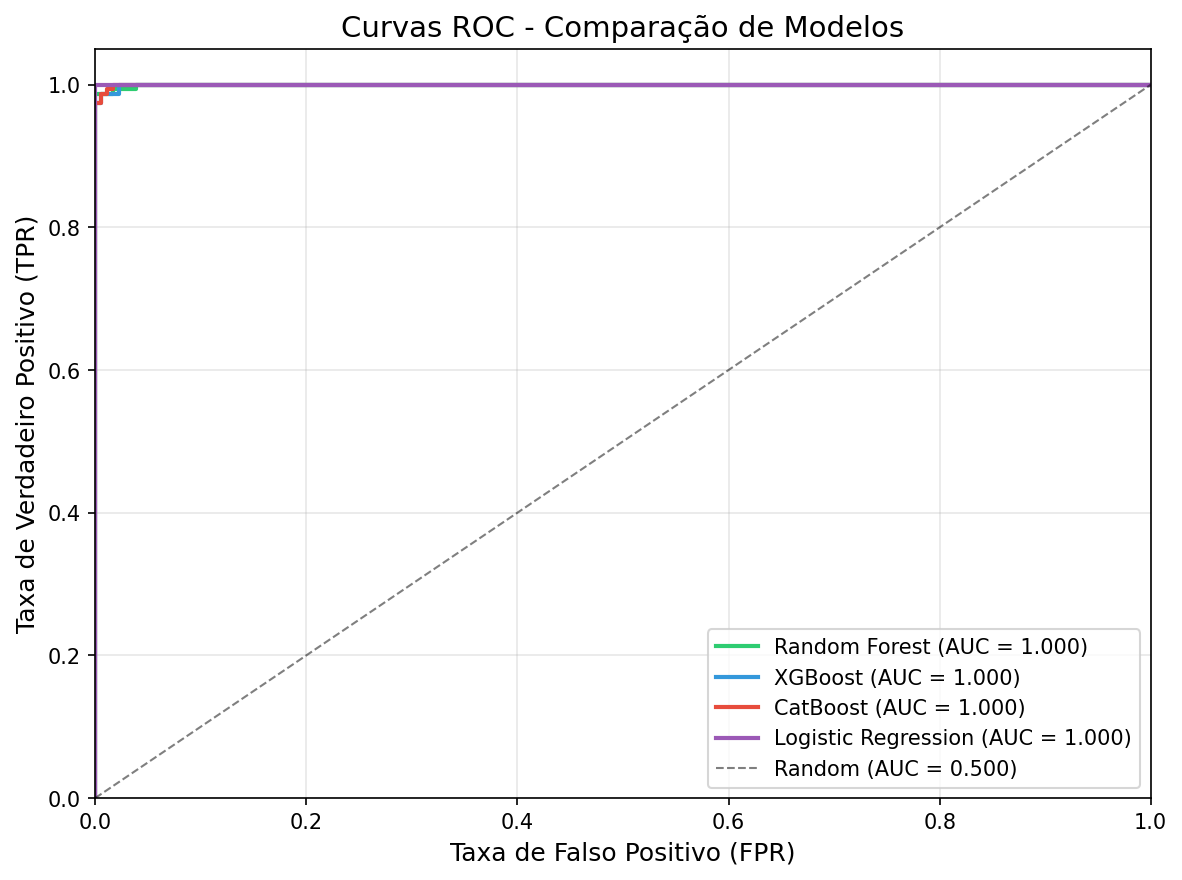
\includegraphics[width=\linewidth]{exp1_roc.png}\\
    {\footnotesize Exp.~1 --- dados mistos.}
    \column{0.5\textwidth}
    \centering
    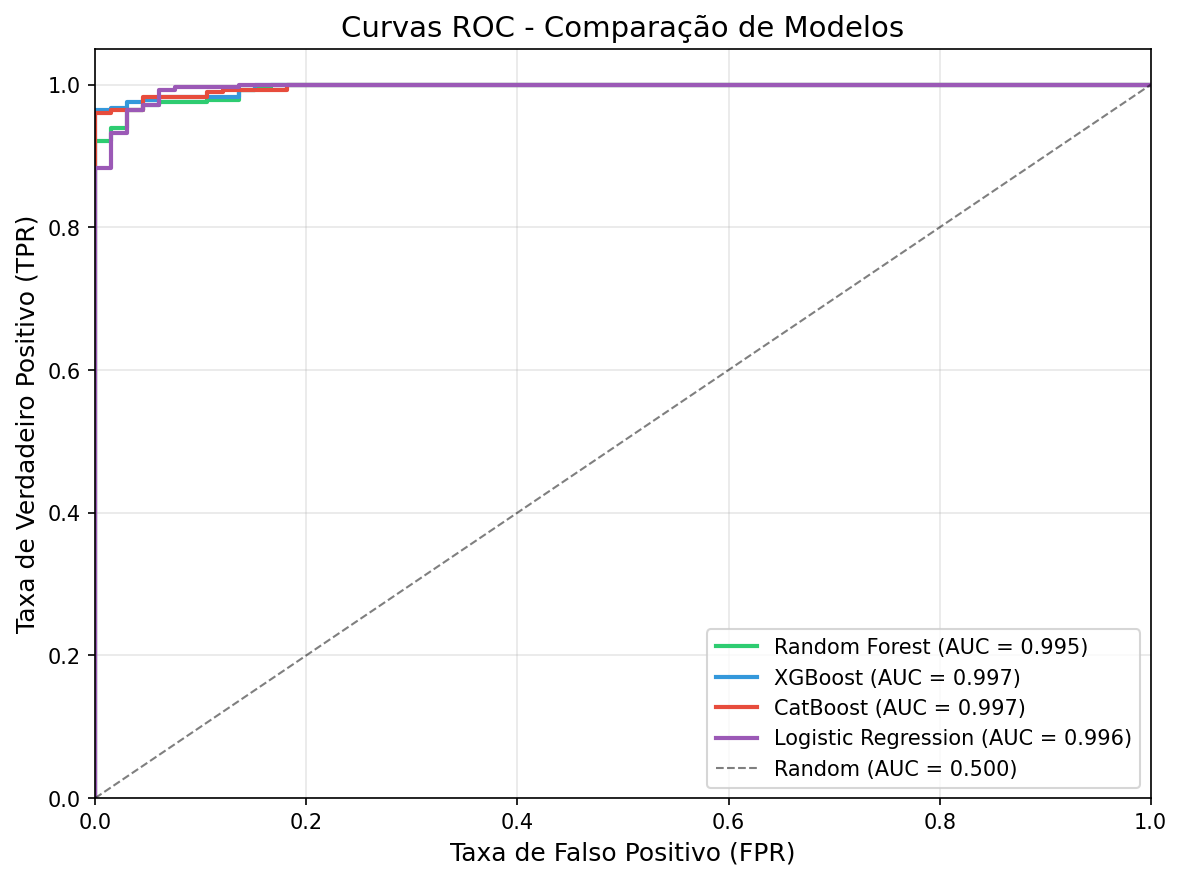
\includegraphics[width=\linewidth]{exp3real_roc.png}\\
    {\footnotesize Exp.~3 --- só curvas reais.}
  \end{columns}
  \vfill
  \centering {\footnotesize Separação quase perfeita no teste misto; leve degradação --- ainda excelente --- no real.}
\end{frame}

\begin{frame}{Custo assimétrico: ajuste do limiar $\tau$}
  \begin{columns}[c]
    \column{0.56\textwidth}
    \centering
    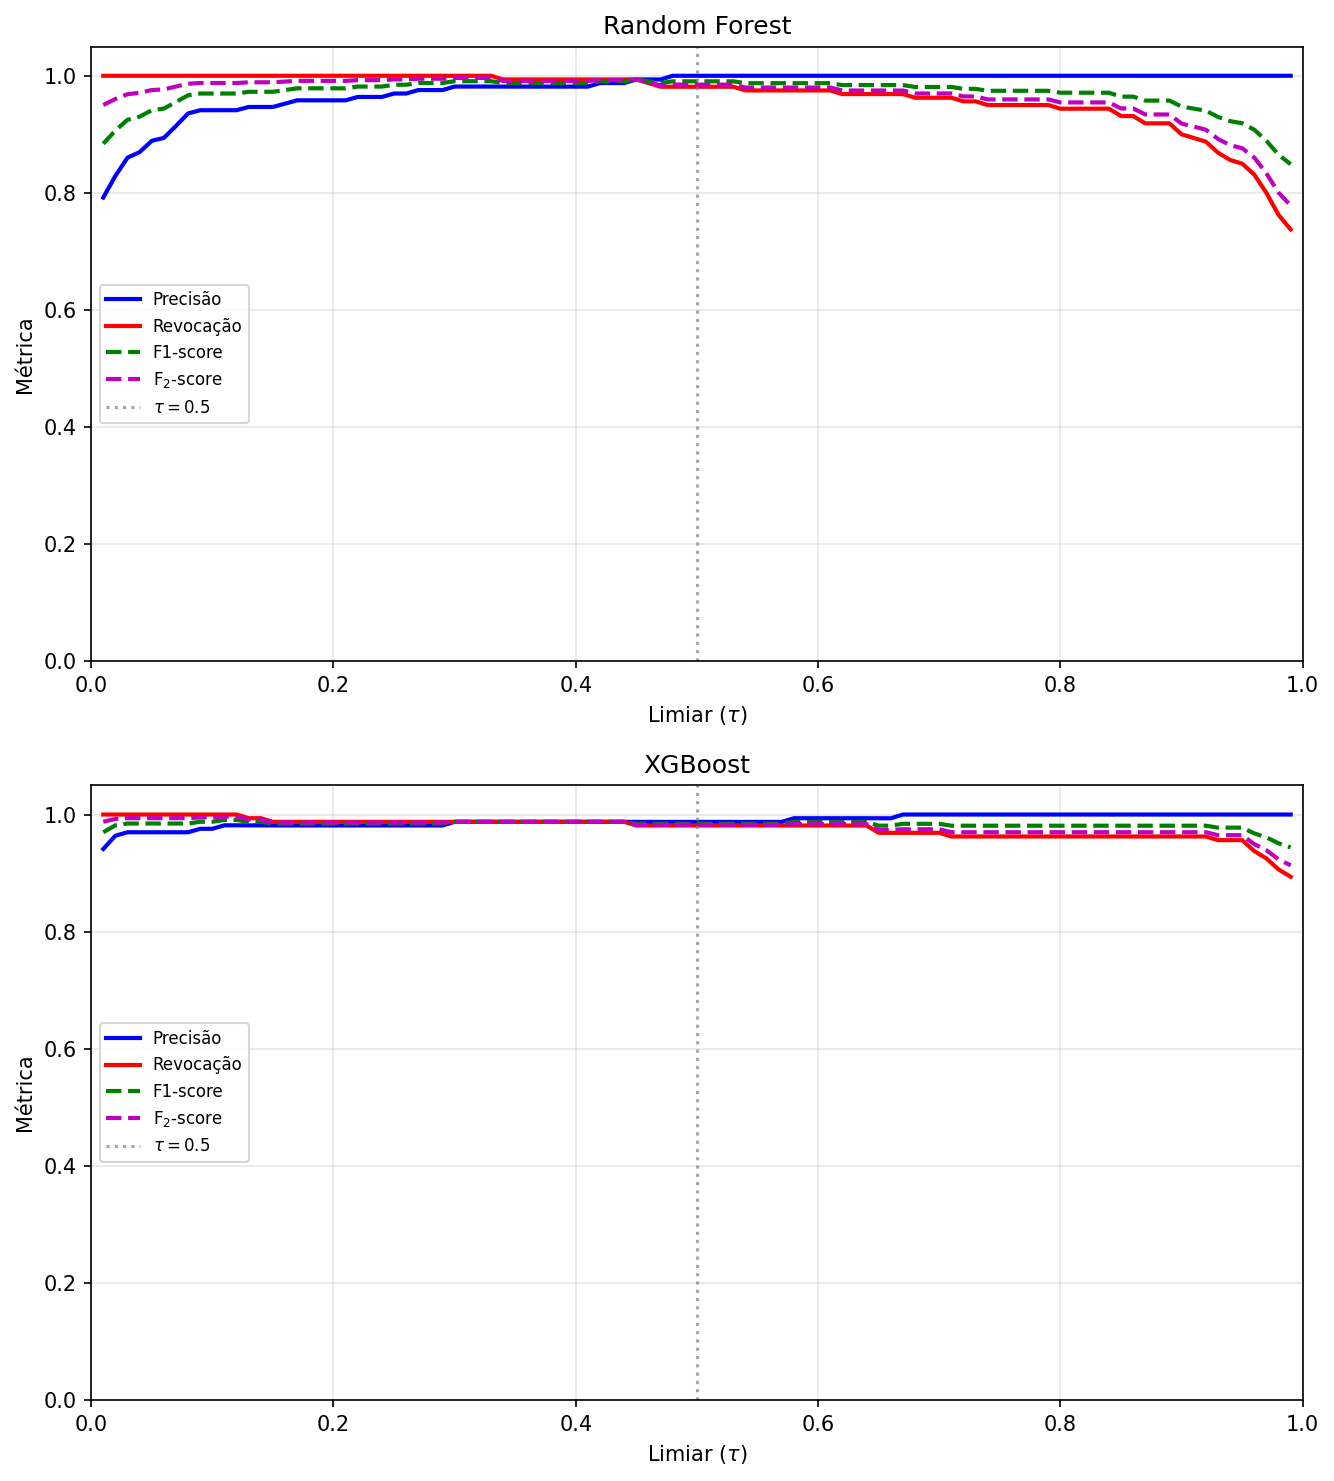
\includegraphics[width=\linewidth]{metrics_vs_threshold.png}
    \column{0.44\textwidth}
    \begin{itemize}\footnotesize
      \item Perder ocultação (FN) $\gg$ revisar alarme falso (FP).
      \item Baixar $\tau$ $\Rightarrow$ \alert{mais sensibilidade}, sem retreinar.
      \item Ajuste de \textbf{pós-processamento}.
    \end{itemize}
  \end{columns}
\end{frame}

% ================================================================ 6. QUAOAR
\section{Estudo de caso: Quaoar}

\begin{frame}{Teste final: uma curva real de Quaoar}
  \begin{itemize}\footnotesize
    \item Dados \alert{externos ao treino} (Gemini, CFHT) --- cedidos por Pereira et al.\ (2023).
    \item Corpo principal $+$ anéis Q1R e Q2R numa só série.
  \end{itemize}
  \centering
  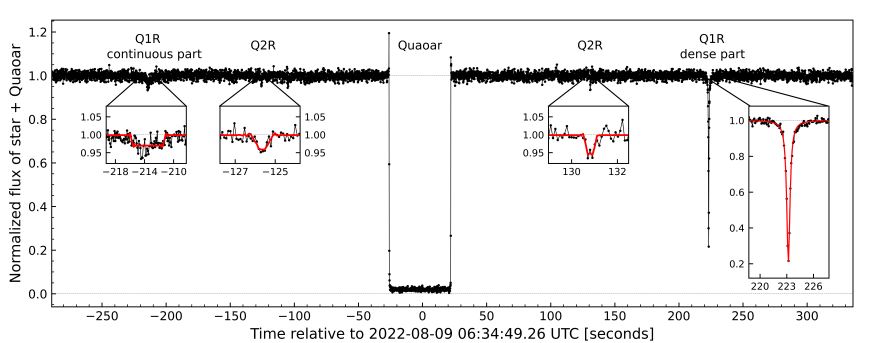
\includegraphics[width=0.93\linewidth]{quaoar_curva.png}
\end{frame}

\begin{frame}{Revisitar por recortes: o achado central}
  \centering
  
\includegraphics[width=0.82\linewidth]{quaoar_recortes.png}
  \vfill
  \begin{columns}[T]
    \column{0.5\textwidth}
    {\footnotesize O anel fino real recebe $\hat{p}\approx 4$--$8\%$ --- baixo em absoluto, \textbf{mas}\dots}
    \column{0.5\textwidth}
    {\footnotesize \dots\ \hl{$\sim$86$\times$} a probabilidade do ruído vizinho ($\sim$0,05\%).}
  \end{columns}
\end{frame}

\begin{frame}{A separação é o que importa}
  \begin{exampleblock}{Com $\tau = 0{,}03$ (em vez de 0,5)}
    \centering
    \textit{Recall} sobre os 4 eventos físicos: \hl{50\% $\rightarrow$ 100\%}\\
    sem \textbf{nenhum} falso alarme nos recortes-controle.
  \end{exampleblock}
  \vfill
  \begin{itemize}\footnotesize
    \item Não é o valor absoluto da probabilidade --- é a \alert{separação} ($\sim$2 ordens de grandeza).
    \item Demonstra, em dado real, a \textbf{revisita de curvas em busca de eventos sutis}.
    \item Janela mais larga \textbf{piora} (causa estrutural: \textit{features} globais) $\to$ trabalho futuro.
  \end{itemize}
\end{frame}

% ================================================================ 7. CONCLUSÕES
\section{Conclusões}

\begin{frame}{Conclusões}
  \begin{itemize}
    \item \textit{Pipeline} interpretável atinge \hl{F1 $\approx$ 0,99}, robusta à simplificação de \textit{features}.
    \item Importância $\neq$ insubstituibilidade (K-means dispensável).
    \item Ajuste de $\tau$ incorpora o custo assimétrico \textbf{sem retreinar}.
    \item Em Quaoar: separa anel real de ruído por \hl{$\sim$2 ordens de grandeza}.
  \end{itemize}
  \vfill
  \begin{block}{Trabalhos futuros}
    \footnotesize Janela deslizante e \textit{features} locais $\bullet$ \textit{holdout} 100\% real $\bullet$
    classificação multi-classe (corpo, anel, atmosfera).
  \end{block}
\end{frame}

\begin{frame}[plain]
  \centering
  \vfill
  {\Large Obrigado.}\\[1em]
  {\large Perguntas?}\\[2em]
  {\footnotesize Thiago Laidler Vidal Cunha --- Observatório Nacional}
  \vfill
\end{frame}

\end{document}
